%% Basierend auf einer TeXnicCenter-Vorlage von Mark M�ller
%%%%%%%%%%%%%%%%%%%%%%%%%%%%%%%%%%%%%%%%%%%%%%%%%%%%%%%%%%%%%%%%%%%%%%%

% W�hlen Sie die Optionen aus, indem Sie % vor der Option entfernen  
% Dokumentation des KOMA-Script-Packets: scrguide

%%%%%%%%%%%%%%%%%%%%%%%%%%%%%%%%%%%%%%%%%%%%%%%%%%%%%%%%%%%%%%%%%%%%%%%
%% Optionen zum Layout des Buchs                                     %%
%%%%%%%%%%%%%%%%%%%%%%%%%%%%%%%%%%%%%%%%%%%%%%%%%%%%%%%%%%%%%%%%%%%%%%%
\documentclass[
paper=a4,							% alle weiteren Papierformat einstellbar
%landscape,						% Querformat
12pt,								% Schriftgr��e (12pt, 11pt (Standard))
BCOR=1cm,							% Bindekorrektur, bspw. 1 cm
%DIVcalc,							% f�hrt die Satzspiegelberechnung neu aus
%											  s. scrguide 2.4
%oneside,							% einseitiges Layout
%twocolumn,						% zweispaltiger Satz
%openany,							% Kapitel k�nnen auch auf linken Seiten beginnen
%halfparskip*,				% Absatzformatierung s. scrguide 3.1
headsepline=true,			% Trennline zum Seitenkopf	
%footsepline,					% Trennline zum Seitenfu�
notitlepage,					% in-page-Titel, keine eigene Titelseite
%chapterprefix,				% vor Kapitel�berschrift wird "Kapitel Nummer" gesetzt
%appendixprefix,				% Anhang wird "Anhang" vor die �berschrift gesetzt 
%normalheadings,			% �berschriften etwas kleiner (smallheadings)
%idxtotoc,						% Index im Inhaltsverzeichnis
%liststotoc,					% Abb.- und Tab.verzeichnis im Inhalt
bibliography=totoc,						% Literaturverzeichnis im Inhalt
%leqno,								% Nummerierung von Gleichungen links
%fleqn,								% Ausgabe von Gleichungen linksb�ndig
%draft,								% �berlangen Zeilen in Ausgabe gekennzeichnet
%cleardoubleplain,    % leere, linke Seite mit Seitenstil 'plain' 
%cleardoubleempty,    % leere, linke Seite mit Seitenstil 'empty'
]
{scrbook}

%\pagestyle{empty}		% keine Kopf und Fu�zeile (k. Seitenzahl)
%\pagestyle{headings}	% lebender Kolumnentitel  

%% Deutsche Anpassungen %%%%%%%%%%%%%%%%%%%%%%%%%%%%%%%%%%%%%
\usepackage[ngerman]{babel}
\usepackage[ansinew]{inputenc}
\usepackage[hypertexnames=false]{hyperref}	% Paket welches die M�glichkeit gibt Links und Verweise innerhalb von PDF Dokumenten zu erzeugen und zu setzen
																						% Ziemlich fr�h Einbinden, sonst werden Abbildungen als Abschnitte via \autoref referenziert.
\usepackage{csquotes}								% Wenn babel verwendet wird mit biblatex, csquotes wird empfohilen zur Darstellung von Anf�hrungszeichen
\usepackage{lmodern} 								% Pixelfreie Schrift
\usepackage{booktabs}								% Tabellen Paket
\usepackage[subfigure]{ccaption}	 
\usepackage{threeparttable} 				% Tabellen Paket um Tabellen mit �berschriften, Fu�noten, ... zu versehen
%\usepackage{a4}	 										% europ�isches A4
\usepackage{courier}								% Stellt Courier New korrekt dar
\usepackage{wasysym}								% Zus�tzliche Symbole wie CheckedBox
\usepackage{marvosym}								% Zus�tzliche Symbole wie CheckedBox
\usepackage{pmboxdraw}							% f�r die Ordnerbaum-Symbole
\usepackage[notext,not1]{stix}			% f�r \boxplus und \boxminus, notext: Text unver�ndert lassen, not1: T1 unver�ndert lassen

%% \autoref Name "`Kapitel"' statt "`Unterabschnitt"'
\addto\extrasngerman{%
\def\subsectionautorefname{Kapitel}%
\def\sectionautorefname{Kapitel}%
}

%% Packages f�r Grafiken & Abbildungen %%%%%%%%%%%%%%%%%%%%%%
\usepackage{graphicx} %% Zum Laden von Grafiken
\usepackage{subfigure} %% Teilabbildungen in einer Abbildung
\newcommand{\subfigureautorefname}{\figureautorefname} % \autoref Name f�r subfigures
%% Beachten Sie:
%% Die Einbindung einer Grafik erfolgt mit \includegraphics{Dateiname}
%% bzw. �ber den Dialog im Einf�gen-Men�.
%% 
%% Im Modus "LaTeX => PDF" k�nnen Sie u.a. folgende Grafikformate verwenden:
%%   .jpg  .png  .pdf  .mps
%% 
%% In den Modi "LaTeX => DVI", "LaTeX => PS" und "LaTeX => PS => PDF"
%% k�nnen Sie u.a. folgende Grafikformate verwenden:
%%   .eps  .ps  .bmp  .pict  .pntg

%% Bibliographiestil %%%%%%%%%%%%%%%%%%%%%%%%%%%%%%%%%%%%%%%%%%%%%%%%%%
\usepackage[
style=authoryear,
natbib,
dashed=false,									% Bei mehreren Werken eines Autors alle einzeln anzeigen
backend=biber, 
block=space										% kleiner horizontaler Platz zwischen den Feldern
]{biblatex}										% Literaturangaben mit BibTeX
\addbibresource{MasterBib.bib}
\setlength{\bibitemsep}{1em}	% Abstand zwischen den Literaturangaben
\setlength{\bibhang}{2em}   	% Einzug nach jeweils erster Zeile

%% Abk�rzungsverzeichnis %%%%%%%%%%%%%%%%%%%%%%%%%%%%%%%%%%%%%
\usepackage{nomencl}					% Paket f�r Abk�rzungsverzeichnis
\makeindex										% Erstellt Masterarbeit.idx welche f�r das Abk�rzungsverzeichnis n�tig ist
															% Muss zwingend VOR \makenomenclature aufgerufen werden!
\let\abk\nomenclature
\renewcommand{\nomname}{Abk�rzungsverzeichnis}  
\setlength{\nomlabelwidth}{0.20\hsize}			  	% Punkte zw. Abk�rzungen und Beschreibung
\renewcommand{\nomlabel}[1]{#1 \dotfill}				
\setlength{\nomitemsep}{-\parsep}								% Zeilenabst�nde verkleinern
\makenomenclature 

%% Quellcode Listings %%%%%%%%%%%%%%%%%%%%%%%%%%%%%%%%%%%%%
\usepackage{listings}
\usepackage[table, dvipsnames]{xcolor}	
\definecolor{KeilGreen}{RGB}{189,249,181}
\definecolor{mygreen}{rgb}{0,0.6,0}
\definecolor{mygray}{rgb}{0.5,0.5,0.5}
\definecolor{mymauve}{rgb}{0.58,0,0.82}

% Style f�r C++
\lstdefinestyle{customcpp}{
  belowcaptionskip=1\baselineskip,
  breaklines=true,
  frame=none,
  xleftmargin=\parindent,
  language=C,
	numbers=left,                    % where to put the line-numbers; possible values are (none, left, right)
  showstringspaces=false,
	%numberstyle=\tiny,								% the style that is used for the line-numbers 
  basicstyle=\footnotesize\ttfamily,
  keywordstyle=\bfseries\color{blue!40!black},
  commentstyle=\itshape\color{green!40!black},
  identifierstyle=\color{black},
  stringstyle=\color{orange},
}
\renewcommand{\lstlistingname}{Quelltext}	% �nder den Name von "`Listing"' auf Quelltext
\newcommand{\lstnumberautorefname}{Zeile}

% Warning, dass mehrere pdfs auf einer Seite sind unterdr�cken
\pdfsuppresswarningpagegroup=1
\pdfminorversion=7

%%%%%%%%%%%%%%%%%%%%%%%%%%%%%%%%%%%%%%%%%%%%%%%%%%%%%%%%%%%%%%%%%%%%%%%
%% Buch                                                              %%
%%%%%%%%%%%%%%%%%%%%%%%%%%%%%%%%%%%%%%%%%%%%%%%%%%%%%%%%%%%%%%%%%%%%%%%
\begin{document}

%%%%%% Titelseite %%%%%%
%Titelseite zentrieren
\newlength\oddsidemarginorig				
\oddsidemarginorig=\oddsidemargin
\advance\oddsidemargin\evensidemargin
\divide\oddsidemargin by 2

%Layout und Text f�r Titelseite
\begin{titlepage}
\begin{center}
\vspace*{0cm}
\hrulefill \\
\vspace*{0.5cm}
\textbf{\LARGE Model Driven Software Engineering \\ mit IBM Rational Rhapsody \\ f�r Embedded Systems \\}	
\vspace*{0.5cm}
%{\bf \huge zum Wintersemester 2012/2013\\}	
\hrulefill \\
\vspace*{1.6cm}
\textbf {\Large Masterprojekt \\}
\vspace*{2cm}
{\large Thomas Sauter \\ Matrikel-Nr.: 3122629\\ Studiengang: SYE\verb|\|2 \\}
\vspace*{1cm}
{\large Hochschule Ulm \\ Graduate School \\ Studiengang Systems Engineering und Management \\}
\vspace*{1cm}
%{\large Firma EvoBus GmbH in Neu-Ulm\\}
\vspace*{1cm}
\textbf{\Large \today \\}
\end{center}
\vspace*{\fill}
\noindent \underline{Betreuer:} \\
																Prof. Dr. Marianne von Schwerin, Hochschule Ulm \\
																%Prof. Dr. Norbert Normann, Hochschule Ulm \\
																%Dipl.-Ing. Alexander Schuh, EvoBus GmbH \\
\end{titlepage}

\cleardoublepage				% mit neuer ungerader Seite weiter
\frontmatter						% ab hier r�mische Nummerierung

%%%%%% Inhaltsverzeichnis %%%%%%
\tableofcontents				% Inhaltsverzeichnis
\cleardoubleoddpage			% Sorgt daf�r, dass die �nderung der Seitennummerierung
												% immer auf einer neuen (rechten) Seite beginnt!
\mainmatter							% ab hier arabische Nummerierung

%% Der Text %%%%%%%%%%%%%%%%%%%%%%%%%%%%%%%%%%%%%%%%%%%%%%%%%%%%%%%%%%%
\chapter{Einleitung}

\section{Motivation}

Das Programmieren von Software kann derzeit in vier Generationen eingestuft werden \parencite{ModelingEmbeddedSystems}. Dabei repr�sentiert die erste Generation die Maschinensprache. Zwar findet die Maschinensprache noch heute Anwendung in allen Prozessoren, allerdings ist das Schreiben von Maschinensprache als bin�rer oder hexadezimaler Code �u�erst m�hselig und fehleranf�llig. 

Deshalb wurde mit der zweiten Generation die Assemblersprache eingef�hrt. Dabei �bersetzt ein Computerprogramm, der Assembler, die Assemblersprache in Maschinensprache. Einheitliche Befehle in Textform erm�glichen ein schnelleres und besser Verst�ndnis daf�r, was ein Programm tats�chlich ausf�hrt. Fehler k�nnen dennoch vorkommen, allerdings nicht mehr in einfachen Konstrukten.Schlie�lich wurden die Programme in Assemblersprache mit zunehmender Dauer gr��er und un�bersichtlicher, wodurch deren Wartung und Test immer schwerer wurde. 

Die h�heren Programmiersprachen wie C oder C++ l�uteten daraufhin die dritte Generation ein, die bis heute Verwendung findet. Die abstrakte Syntax ist eher an menschliche Gewohnheiten angepasst und beschreibt, wie ein Problem gel�st wird. Ein Compiler �bersetzt den Quellcode in Maschinensprache. Aber auch hier w�chst die Software kontinuierlich, wodurch erneut das Problem der Komplexit�t auftritt. Das spiegelt sich auch in einer Umfrage von \citet[Folie 48]{EmbeddedMarketsStudy} wider. Dort wird die steigende Komplexit�t, verbunden mit der zunehmenden Anzahl an Codezeilen, als gr��te Herausforderungen im kommenden Jahr in der Entwicklung von Software f�r Embedded Systems angegeben.

Abhilfe sollen die Sprachen der vierten Generation schaffen, wobei die Literatur die Inhalte der vierten Generation nicht klar abgrenzt. Nach \citet{ModelingEmbeddedSystems} geh�rt zur vierten Generation auch die Modellierungssprache UML. Die UML hebt die Programmierung nochmals auf eine h�here Abstraktionsebene und versucht so die Komplexit�t zu bew�ltigen. Dabei kommen standardisierte Modellelemente zum Einsatz, die eine h�here Informationsdichte haben als �bliche Programmiersprachen. Mit den Modellelementen k�nnen Grafiken wie Klassen-, Sequenz- und Zustandsdiagramme modelliert werden. Oft ist es noch g�ngige Praxis, dass UML-Modelle lediglich zur Dokumentation verwendet werden. Dabei wird aber nicht das gesamte Potential der UML ausgenutzt. Zusammen mit einem Codegenerator entwickelt sich die UML zu einer leistungsstarken Modellierungssprache, bei der das Programmieren vom Modellieren abgel�st wird. In diesem Zusammenhang ist eine Entwicklungsumgebung, welche das automatisierte Generieren von Quellcode unterst�tzt, unverzichtbar. Bezogen auf die vier Generationen �berf�hrt der Codegenerator das UML-Modell aus der vierten Generation in ausf�hrbaren Quellcode der dritten Generation.     

\section{Aufgabenstellung}

Der Fokus im Rahmen dieser Arbeit liegt auf der modellbasierten Softwareentwicklung f�r Embedded Systems. Die Basis bildet die Laborveranstaltung zur Vorlesung Embedded Systems. Dort wurde bisher mit Hilfe des Tools IBM Rational Rhapsody und des Willert Realtime RXF aus UML-Modellen Quellcode in C generiert. Der generierte Quellcode wird in der Entwicklungsumgebung Keil uVision kompiliert und auf ein Evaluierungsboard geladen. 

Die erste Aufgabe besteht darin, die bisher existierenden Laboraufgaben von der Programmiersprache C nach C++ zu �berf�hren. Besonderheiten in diesem Zusammenhang stellt das Einbinden externer C-Quellen dar, was im Weiteren Verlauf der Arbeit nochmals thematisiert wird. L�sungen der Laboraufgaben in der Programmiersprache C++ sind nicht Inhalt der vorliegenden Arbeit.

In den existierenden Laboraufgaben wurden bereits verschiedene Peripherieger�te des Evaluierungsboards verwendet, unter anderem LED-Bar, Poti, Display, Joystick und Interrupt-Button. Hier sollen weitere Bauteile angesprochen und die Laboraufgaben erweitert werden. Dabei handelt es sich um folgende Funktionalit�ten:

\begin{itemize}
\item Ethernet-Kommunikation
\item WLAN-Kommunikation
\item Lesen und Schreiben einer SD-Karte
\end{itemize}

Das Hauptaugenmerk bei der Implementierung liegt darauf, dass der generierte C++-Quellcode in Keil uVision nicht mehr ge�ndert werden muss, ansonsten geht der Vorteil der automatisierten Codegenerierung durch Rational Rhapsody verloren. Eine Ausnahme bildet die WLAN-Kommunikation. Da das Evaluierungsboard �ber keine eigene WLAN-Antenne verf�gt, muss diese �ber einen externes WLAN-Modul zur Verf�gung gestellt werden. Zwar erfolgt die Implementierung f�r das Evaluierungsboard �ber die bestehende Toolkette, jedoch ben�tigt das externe WLAN-Modul eine spezifische Entwicklungsumgebung in welcher der entsprechende Code von Hand implementiert wird.

Den Abschluss der Arbeit bildet die Verifikation. Dabei soll auch ein modellbasierter Test implementiert werden. Rational Rhapsody bietet dazu die Erweiterung TestConductor an, welche diese Funktionalit�t unterst�tzt. Damit aus den modellierten Testf�llen ausf�hrbarer Quellcode entstehen kann, wird ebenfalls das Willert Realtime RXF sowie Keil uVision ben�tigt. Zu Beginn der Arbeit war geplant, dass die Implementierungen zu den neuen Funktionen einem modellbasierten Test unterzogen werden. Allerdings existiert derzeit kein Willert Realtime RXF, das die verwendete Toolchain und den TestConductor unterst�tzt, sowie C++-Quellcode generiert. Ein Release eines entsprechenden Willert Realtime RXF ist f�r das vierte Quartal im Jahr 2017 vorgesehen. Aus diesem Grund soll eine der bereits existierenden Laboraufgaben in C verwendet werden und exemplarisch ein Testszenario modelliert werden.

\chapter{Entwicklungsumgebung}

\section{Hardware}

\subsection{Evaluation Board Keil MCB1760}
Das Keil MCB1760 Evaluation Board enth�lt einen NXP LPC1768 Mikrocontroller basierend auf einem  100Mhz ARM 32-bit Cortex-M3 Mikroprozessor. Neben den wesentlichen Komponenten und Schnittstellen, welche in \autoref{fig:MCB1760EvalBoard} dargestellt sind, verf�gt das Keil MCB1760 Evaluation Board �ber 512KB Flash und 64KB RAM Speicher.

\begin{figure}[ht!]
	\centering
	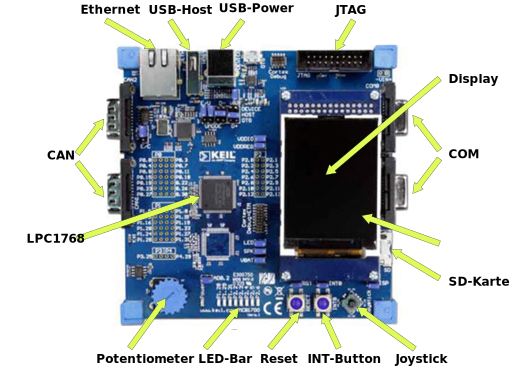
\includegraphics[width=1\textwidth]{images/MCB1700.pdf}
	\caption{Komponenten des MCB1760 Evaluation Board.}
	\label{fig:MCB1760EvalBoard}
\end{figure}

In der Regel werden Evaluation Boards in fr�heren Entwicklungsphasen eingesetzt, um die Leistungsgrenzen der gew�hlten Architektur zu verifizieren. Im Rahmen dieser Arbeit steht die Integration des Evaluation Boards zusammen mit der Toolchain im Vordergrund. 

\subsection{WLAN-Modul ESP8266}

\begin{figure}[b!]
	\centering
		\includegraphics[width=1\textwidth]{images/ESP8266_E12.pdf}
		\caption{WLAN-Modul ESP8266.}
	\label{fig:ESP8266}
\end{figure}

Das WLAN-Modul ESP8266 ist eines von wenigen Boards auf dem Markt, das �ber einen Mikrocontroller mit WLAN-Funktionalit�t verf�gt. Das Herzst�ck des Mikrocontrollers ist der bis zu 160MHz schnelle 32-bit Xtensa LX106 Mikroprozessor von Tensilica. Dabei gibt eine ganze Reihe von Boards, die sich vor allem in ihrer Dimension, den damit zug�nglichen Pins und dem Flash Speicher unterscheiden. Im Rahmen dieser Arbeit wird das Board ESP8266-12E verwendet, wie es in \autoref{fig:ESP8266} dargestellt ist. Das Board verf�gt �ber 4MB Flash und 65KB RAM Speicher. Eine hohe Popularit�t im Internet erlangte das Board auch unter dem Begriff \textit{NodeMCU}. Der Name \textit{NodeMCU} stammt dabei von der Firmware, die ab Werk vorinstalliert ist. Die Open-Source Firmware basiert auf der Skriptsprache Lua. In dieser Arbeit wird die Firmware \textit{NodeMCU} nicht verwendet, weshalb das Board im Weiteren auch als WLAN-Modul ESP8266 bezeichnet wird. Die Programmierung �ber Lua-Skripte ist m�glicherweise komfortabler, bietet aber eine wesentlich geringere Flexibilit�t als eine Programmiersprache wie C. 

Der gro�e Vorteil des verwendeten Boards liegt in der USB-Schnittstelle. Diese dient als Programmier-Schnittstelle und Spannungsversorgung zugleich.  Dabei wird die USB-Schnittstelle durch den USB/UART-Wandler CH340G und eine Spannungsstabilisierung unterst�tzt. Das vereinfacht die Programmierung des ESP8266, da nicht beachtet werden muss, dass bestimmte Pins vor der Programmierung definierte Pegel haben. Zudem muss keine explizite Spannungsversorgung entwickelt werden. 

\section{Software}

\subsection{IBM Rational Rhapsody}

Derzeit gibt es auf dem Markt eine Vielzahl an Software-Modellierungswerkzeuge, die sich im Wesentlichen durch ihre Funktionen und den daraus resultierenden Preis unterscheiden. Jedoch haben die meisten dieser Tools miteinander gemein, dass sie die Modellierungssprache UML unterst�tzen. So gibt es unter anderem einige kostenlose Tools wie StarUML oder Netbeans, die geringen Anforderungen durchaus gen�gen. Weitaus m�chtiger sind etwa Enterprise Architect von SparxSystems und das in dieser Arbeit verwendete Rational Rhapsody von IBM. Mit Rational Rhapsody ist es m�glich, nebem UML-Modellierung weitere Aufgaben zu bearbeiten, die w�hrend der Softwareentwicklung anfallen. Beispielsweise k�nnen Anforderungen direkt spezifiziert oder auch aus DOORS NG importiert und zu der erstellten Architektur verlinkt werden. Ein Codegenerator �bersetzt die Architektur in Quelltext. Dabei bietet der Codegenerator etliche Konfigurationsm�glichkeiten, um Layout und Syntax nach Belieben anzupassen. Das Spezifizieren und Ausf�hren von Tests in einer integrierten Testumgebung runden den Funktionsumfang zur Unterst�tzung eines Software Entwicklungsprozesses ab.

Rational Rhapsody wird in verschiedenen Versionen Angeboten, die sich stark in ihrem Funktionsumfang unterscheiden. Grundlegende Funktionen, wie etwa das Erstellen von UML-Diagrammen und das Verlinken von Anforderungen ist mit allen Versionen m�glich. Weitere Funktionalit�ten wie grafikbasierte Simulation oder  
automatische Codegenerierung, unter anderem auch f�r Embedded Echtzeitsysteme, ist nur in den Premium-Versionen verf�gbar \parencite{IBM2017}. 

Beim Generieren von Quelltext unterst�tzt Rational Rhapsody die Programmiersprachen C, C++, Java und C\#. Dabei ist es wichtig, dass direkt beim Anlegen des Projekts die gew�nschte Programmiersprache ausgew�hlt wird. Denn in der Folge startet Ratioal Rhapsody beim �ffnen der Rhapsody Projektdatei stets die passende Variante f�r die definierte Programmiersprache. Da die Implementierungen in dieser Arbeit in C++ erfolgen, ergibt sich somit die Version \textit{IBM Rational Rhapsody Developer for C++}, die zudem den vollen Funktionsumfang beinhaltet. 

\subsubsection*{Rhapsody TestConductor Add On}

Der Rhapsody TestConductor ist Teil der Testumgebung von Rational Rhapsody, welche auf drei Hauptkomponenten basiert:

\begin{itemize}
\item Automatisiertes Generieren von Test-Architekturen
\item Automatisiertes Generieren von Testf�llen
\item Automatisiertes Ausf�hren von Testf�llen
\end{itemize}

Dabei unterst�tzt der TestConductor in der Basisversion das automatisierte Generieren von Test-Architekturen, sowie das Ausf�hren von Testf�llen. Mit der Erweiterung Automatic Test Generation (ATG) wird auch das automatisierte Generieren von Testf�llen unterst�tzt. Ungeachtet dessen steht im Fokus des TestConductors der modellbasierte, dynamische Test. So erm�glicht der TestConductors das Modellieren von Testf�llen in Form von Sequenz-, Zustands- und Aktivit�tsdiagrammen. Zus�tzlich ist es aber auch m�glich, Testf�lle als Quellcode zu implementieren.

Dar�ber hinaus bringt der TestConductor das Rhapsody UML Testing Profile mit sich, basierend auf dem offiziellen UML Testing Profile der \citet{OMGUMLTestingProfile}. Dabei gilt es zu beachten, dass das Rhapsodoy UML Testing Profile nicht alle Elemente des UML Testing Profiles enth�lt. Aber es verf�gt �ber zus�tzliche Elemente, die nicht Teil des UML Testing Profiles der OMG sind. Ein Beispiel daf�r sind Platzhalter f�r Schnittstellen, die nicht Teil der zu testenden Komponente sind \parencite{TestConductorAddOn}. 

\subsection{Willert Embedded UML RXF}
Der generierte Code aus Rhapsody eignet sich zun�chst nicht zur Ausf�hrung auf einem Target. Die UML-Notation ist viel leistungsst�rker und auf einer h�heren Abstraktionsebene als jede h�here Programmiersprache. UML-Elemente wie asynchrone Kommunikation, aktive Klassen oder auch komplexe Zust�nde k�nnen nicht direkt in eine h�here Programmiersprache �bersetzt werden. 

Das Tool Embedded UML Real-time eXecution Framework (RXF)\abk{$RXF$}{Real-time eXecution Framework} der Firma Willert bildet die Schnittstelle zwischen UML-Modell und einer Zielplattform bestehend aus Compiler, CPU\abk{$CPU$}{Central Processing Unit} und einem m�glichen RTOS\abk{$RTOS$}{Real Time Operating System}. Durch eine Abstraktionsschicht werden die g�ngigsten Echtzeit-Betriebssysteme auf dem Markt unterst�tzt. Das bedeutet, dass in UML definierte Timer oder Events unabh�ngig vom Betriebssystem verwendet werden k�nnen. Somit ist das Software-Design komplett losgel�st vom gew�hlten Target.

Bei der Codegenerierung unterst�tzt das RXF die beiden bekanntesten UML-Tools, Rhapsody und Sparx Enterprise Architect, sowie eine Vielzahl an IDEs\abk{$IDE$}{Integrated Development Environment}. Um eine bestm�gliche Integration zu gew�hrleisten, ist jede Variante des RXF auf die verwendete Toolchain zugeschnitten. Ein Vorteil davon ist, dass die Target IDE �ber das RXF mit Rhapsody verbunden ist und somit der Code aus dem UML-Modell direkt in die Target IDE generiert wird \parencite{ModelingEmSys}. Zur Unterscheidung der vielen verschiedenen Varianten hat die Firma Willert mit der Version 6 einen Produktcode eingef�hrt, welcher zur Identifikation der enthaltenen Komponenten dient. Das Schema ist in \autoref{tab:WillertProduktcode} abgebildet.

\begin{table}[!b]
\centering
\small
	\begin{threeparttable}
	\begin{tabular}{c|c|c|c|c|c}
		\toprule
			 UML-Tool & Programmiersprache & RTOS & Compiler & EvalBoard\tnote{*} & Erweiterungen\tnote{**}\hspace{1ex} \\
		\bottomrule
		\end{tabular}
		\begin{tablenotes}
			\footnotesize 
			\item[*]{Die EvalBoard Komponente ist kein Teil des Produkts. Sie sagt lediglich aus, mit welcher CPU Familie das Produkt verwendet werden kann.}
			\item[**]{Erweiterungen sind optional und k�nnen auch miteinander kombiniert werden. M�gliche Zus�tze sind "`TD"' f�r Embedded UML Target Debugger, "`TC"' f�r Test Conductor oder "`Eval"' f�r eine RXF Evaluierungsversion.}
		\end{tablenotes}
	\end{threeparttable}
	\caption{Produktcode zur Identifikation der enthalten Komponenten \parencite{RXFMigrationGuide}.}
	\label{tab:WillertProduktcode}
\end{table}

In dieser Arbeit wurden die Varianten \begin{itshape}RXF-Eval\_Rpy-Cpp-ARM\end{itshape} in der Version 6.02 und \begin{itshape}Rpy\_CPP\_CMSIS\_Keil5\_ARM\_MCB1700\_TD\end{itshape} in der Version 6.01 verwendet.

\subsection{Keil uVision}
Die IDE Keil uVision ist Teil des Keil Microcontroller Development Kit (MDK)\abk{$MDK$}{Microcontroller Development Kit}. Es vereint einen Projektmanager und eine Run-Time Environment (RTE)\abk{$RTE$}{Run-Time-Environment}, mit deren Hilfe vorgefertigte Software Pakete integriert werden k�nnen. Die Software Pakete k�nnen Bibliotheken, Module, Konfigurationsdateien, Templates und Dokumentation enthalten, welche bei der Inbetriebnahme des Targets unterst�tzen. Die Basisfunktionalit�ten einer gew�hnlichen IDE, wie Quellcode-Editor und Debugger, sind ebenfalls enthalten \parencite{MDK}.

In dieser Arbeit wird das Keil MDK in der Version 5 verwendet. Im Vergleich zum vorherigen Keil MDK in der Version 4, ist eine wesentliche Neuerung das Echtzeitbetriebssystem Cortex Microcontroller Software Interface Standard (CMSIS)\abk{$CMSIS$}{Cortex Microcontroller Software Interface Standard}. Es l�st das bisherige RTX Real-Time Library (RL-ARM)\abk{$RL-ARM$}{Real-Time Library for ARM microprocessors} Echtzeitbetriebssystems ab und bringt die folgenden Vorteile mit sich \parencite{RLARMtoCMSIS}: 

\begin{itemize}
\item Standardisierte API
\item Basisfunktionen zur Unterst�tzung von UML oder Java
\item Einfaches wiederverwenden von Software Komponenten durch einheitliche Funktionen
\item CMSIS konforme Middleware kann einfach angepasst werden
\end{itemize}

\subsection{Arduino IDE}

Um das WLAN-Modul ESP8266 in der Programmiersprache C zu implementieren, wird die Arduino IDE verwendet. Zwar bringt die Ardunio IDE nur einen sehr geringen Funktionsumfang mit sich, so ist beispielsweise kein Debugger enthalten. Der fehlende Debugger kann durch Ausgaben auf die serielle Schnittstelle teilweise kompensiert werden, dazu bietet die Arduino IDE auch ein integriertes Terminal an. Dennoch ist die Arduino IDE weit verbreitet und kostenlos, zudem ist sie �berschaubar und daher sehr schnell zu beherrschen. Nach der Installation unterst�tzt die Arduino IDE eine Vielzahl an Ardunio-Boards, jedoch nicht das WLAN-Modul ESP8266. Dazu muss die Arduino IDE um das ESP8266-Paket erweitert werden. Eine detaillierte Installationsanleitung beschreibt \citet{ESP8266Sauter17}. Der Quellcode ist einem sogenannten Sketch enthalten, welcher die beiden klassischen Funktionen \textit{setup} und \textit{loop} implementiert.

\chapter{Implementierungen}
\section{Ethernet}

Dieses Kapitel beschreibt die Einbindung der Ethernet Schnittstelle des Keil MCB1760 Evaluation Boards. Ziel ist es, dass zwei Boards �ber ihre Ethernet Schnittstelle Daten austauschen k�nnen. In der Implementierung nach \citet{Steinmeyer} wurde die gew�nschte Funktionalit�t bereits umgesetzt, jedoch auf der Basis des RTX RL-ARM Echtzeitbetriebssystems und einer damit �berholten Version der Keil MDK. Zudem soll die gesamte Implementierung in Rhapsody stattfinden, so dass der generierte Code in der IDE Keil uVision lediglich �bersetzt und auf das Target geflasht werden muss. 

Zur Implementierung und Demonstration der Kommunikation �ber Ethernet wurde eine Entwicklungsumgebung entsprechend der nachfolgenden Abbildung aufgebaut.

\begin{figure}[h!]
	\centering
		\includegraphics[width=1\textwidth]{images/EthernetAufbau.pdf}
		\caption[Demonstrator Ethernet zwischen zwei Eval Boards]{Demonstrator f�r die Kommunikation zwischen zwei MCB1760 Evaluation Boards �ber Ethernet}
	\label{fig:DemonstratorEthernet}
\end{figure}

Wie in \autoref{fig:DemonstratorEthernet} dargestellt, sind die beiden MCB1760 Evaluation Boards �ber Patchkabel mit einen Hub verbunden. Der Hub hat gegen�ber einem Switch oder Router den Nachteil, dass er eine geringere nutzbare Bandbreite mit sich bringt. Grund daf�r ist, dass der Hub ein Datenpaket immer an jedes angeschlossene Ger�t sendet, unabh�ngig davon, ob das Datenpaket an das Ger�t adressiert wurde oder nicht. Jedoch unterst�tzt dieses Defizit bei der Implementierung, indem mit Hilfe eines PCs das Tool Wireshark den Datenverkehr zwischen den beiden MCB1760 Evaluation Boards abh�rt. Da die versendeten Datenpakete eine Gr��e von zwei Bytes haben, spielt die nutzbare Bandbreite im Rahmen dieser Arbeit keine Rolle. 

\subsection{Anforderungen}\label{subsec:Anforderungen} 

Zur Demonstration einer funktionsf�higen Ethernet-Kommunikation soll ein exemplarisches Szenario implementiert werden. So sollen LEDs durch den Joystick auf dem jeweils anderen Board ein- und ausgeschaltet werden. Dabei soll die Position des Joysticks angeben, welche LED die LED-Bar ein- oder ausschaltet. Des Weiteren soll das Display die zuletzt empfangene Position anzeigen. Damit die MCB1760 Evaluation Boards einfach zu identifizieren sind, soll das Display zudem die Host IP Adresse sowie die Target IP Adresse darstellen. Beim Senden sowie beim Empfangen eines Datenpakets soll der Transmitter bzw. der Receiver kurzzeitig eine LED blinken lassen. Die Zuordnung von Funktionen zu den LEDs der LED-Bar ist \autoref{fig:Szenario} rechts dargestellt. 

\begin{figure}[h!]
	\centering
		\includegraphics[width=1\textwidth]{images/Szenario.pdf}
		\caption[Beispiel mit Zuordnung der LEDs]{Beispiel mit Zuordnung der LEDs.}
	\label{fig:Szenario}
\end{figure}

Zudem veranschaulicht \autoref{fig:Szenario} das Funktionsprinzip. Auf dem Host MCB1760 Evaluation Board bewegt der Benutzer den Joystick in die linke Richtung. Das f�hrt dazu, dass beim Remote MCB1760 Evaluation Board die Receiver LED P1.29 kurzzeitig aufleuchtet, sowie die LED P2.3 dauerhaft angeschaltet wird. Bewegt der Benutzer den Joystick erneut in die linke Richtung, erlischt die LED P2.3 wieder.

\subsection{Architektur}
Bei der Formulierung der Anforderungen in \autoref{subsec:Anforderungen} wurde darauf geachtet, dass diese in m�glichst aktiver Form spezifiziert sind. Dadurch k�nnen die ben�tigten Klassen abgeleitet werden, welches sich im Folgenden durch die �hnlichkeit von Subjekten oder Objekten zu den Klassennamen widerspiegelt.

Die Architektur der Ethernet-Kommunikation ist als Klassendiagramm in \autoref{fig:ClassDiagramEthernet} dargestellt. Zentrales Element ist die Basisklasse \texttt{Ether\-net\-Con\-trol\-ler}, von ihr werden die beiden Klassen \texttt{Ether\-net\-Transmitter} und \texttt{Ether\-net\-Receiver} abgeleitet. Diese beiden Klassen arbeiten in separaten Tasks und sind f�r das Senden und Empfangen von Datenpaketen verantwortlich. Auf der linken Seite in \autoref{fig:ClassDiagramEthernet} sind die Klassen \texttt{Running\-Indicator\-Led} und \texttt{Joystick} abgebildet, welche ebenfalls in eigenen Tasks ausgef�hrt werden. Die Klasse \texttt{Running\-Indicator\-Led} l�sst die LED P1.31 zyklisch blinken, mit einer Periodendauer von einer Sekunde. Sie dient zu Debugging zwecken und um unmittelbar zu erkennen, ob das Target l�uft. Die Klasse \texttt{Joystick} pollt regelm��ig die Position des Joysticks. Auf der rechten Seite sind die Klassen \texttt{LedBar}, \texttt{Display} und \texttt{Led} zu finden. Dabei liegt zwischen den Klassen \texttt{LedBar} und \texttt{Led} eine Komposition mit der Multiplizit�t vier vor, wodurch der LED-Bar die LEDs zugeordnet sind, welche eine Joystick Position repr�sentieren. Au�erhalb des Pakets \texttt{DefaultPkg} sind Abh�ngigkeiten zu externen Bibliotheken in orange eingezeichnet. Die verwendeten Bibliotheken, Network und Graphics Component, stammen aus der MDK Middleware und vereinfachen das Verwenden dieser Peripherieger�te. M�gliche Vorgehensweisen beim Einbinden externer Quellen beschreiben \citet{ExternalSources}.

\begin{figure}[h!]
	\centering
		\includegraphics[width=1\textwidth]{images/ClassDiagramEthernet.pdf}
		\caption[Klassendiagramm Ethernet-Kommunikation]{Klassendiagramm zur Ethernet-Kommunikation. Klassen, die in eigenen Tasks laufen sind rot eingezeichnet.}
	\label{fig:ClassDiagramEthernet}
\end{figure}

\subsection{Design und Coding}\label{subsec:DesignUndCoding}
In diesem Kapitel werden Attribute, Funktionen und Statecharts wichtiger Klassen im Detail vorgestellt.

\subsubsection*{Ethernet-Controller, Transmitter und Receiver}
Der Ethernet-Controller basiert auf der MDK Middleware Network Component in der Version 7.4.0. Die Network Component beinhaltet eine Vielzahl an Services, Sockets (TCP, UDP und BSD), sowie eine Ethernet Schnittstelle inklusive eines IPv4/IPv6 Protocol Stacks. In dieser Arbeit wird der BSD Socket als Datagram Socket (UDP) zusammen mit dem IPv4 Protocol Stack verwendet. Der BSD Socket stellt eine API zur Verf�gung, die das Aufbauen und Abhandeln einer Netzwerkkommunikation unterst�tzt. Urspr�nglich wurden die BSD Sockets f�r unixnahe Betriebssysteme entwickelt. Mittlerweile sind sie in den POSIX Standard aufgenommen und wurden auch von Microsoft Windows �bernommen. Ein Vorteil der BSD Sockets ist, dass mit geringem Konfigurationsaufwand zwischen Stream Sockets (TCP) und Datagram Sockets (UDP) gewechselt werden kann. 

Die Klasse \texttt{Ether\-net\-Con\-trol\-ler} mit ihren Attributen und Operationen ist in \autoref{fig:EthernetController} dargestellt. Zum Spezifizieren der IP-Adressen dienen die Attribute \texttt{hostIpAddr} und \texttt{remoteIpAddr} vom Typ String. Die IP-Adresse werden in Rhapsody �ber den Features Dialog der beiden Attribute initial festgelegt. Zum Flashen des zweiten Targets k�nnen die IP-Adressen einfach getauscht werden.

\begin{figure}[h!]
	\centering
		\includegraphics[width=0.475\textwidth]{images/EthernetController.pdf}
		\caption{Basisklasse des Ethernet-Controllers mit abgeleiteten Klassen.}
	\label{fig:EthernetController}
\end{figure}

\lstset{escapechar=@, escapeinside={(*@}{@*)}, style=customcpp}
\begin{lstlisting}[caption={Konstruktor des Ethernet-Controllers}, label={lst:EthernetControllerConstructor}, captionpos=b]
unsigned char buf[8];

if (status != netOK)   
{	
	// Initialize the network component only once
	status = netInitialize (); (*@\label{netInitialize}@*)

	// Set the host ip address once
	netIP_aton (hostIpAddr, NET_ADDR_IP4, buf);
	netIF_SetOption (
		NET_IF_CLASS_ETH | 0, 
		netIF_OptionIP4_Address, 
		buf, NET_ADDR_IP4_LEN);
}
\end{lstlisting}

\autoref{lst:EthernetControllerConstructor} zeigt den Konstruktor des \texttt{Ether\-net\-Con\-trol\-lers}. Der Konstruktor verwendet ausschlie�lich Funktionen der Network Component, was am Prefix \texttt{net} zu erkennen ist. In \autoref{netInitialize} wird die Funktion \texttt{netInitialize} aufgerufen. Diese Funktion muss bei Systemstart einmalig ausgef�hrt werden. Sie initialisiert Systemressourcen, Protokolle und zwei Tasks f�r den Network Core. Bei erfolgreicher Initialisierung wird dem Attribut \texttt{status} der Wert \texttt{netOK} zugewiesen. Mit der �bergeordneten Abfrage wird sichergestellt, dass die Initialisierung auch nur einmalig durchgef�hrt wird, auch wenn der Konstruktor des \texttt{Ether\-net\-Con\-trol\-lers} durch die beiden Instanzen der abgeleiteten Klassen zweimal durchlaufen wird. Die Funktion \texttt{netIP\_aton} konvertiert eine IP-Adresse vom Typ String in eine bin�re Form. Dadurch ist es anschlie�end m�glich, die Host IP-Adresse dynamisch mit Hilfe der Funktion \texttt{netIF\_SetOption} zu setzen. Somit ist die Konfiguration der Host IP-Adresse ebenfalls in Rhapsody m�glich und ben�tigt keine manuelle Anpassung innerhalb der Keil Umgebung.

Das Sequenzdiagramm in \autoref{fig:EthernetTransmitter} stellt das Verhalten des Ethernet-Transmitters dar. Der \texttt{Ether\-net\-Transmitter} erstellt in seinem Konstruktor einen Socket vom Typ Datagram Sockets (UDP), zu erkennen am �bergabeparameter \texttt{SOCK\_DGRAM}. Dem Socket wei�t er durch Aufruf von \texttt{connect} die Remote IP-Adresse, also die IP-Adresse des anderen Endpunkts, zu. Aufgrund des gew�hlten Typ Datagram Sockets (UDP), richtet der \texttt{Ether\-net\-Transmitter} zudem ein Adressfilter zwischen den Endpunkten ein. Im weiteren Ablauf reagiert der \texttt{Ether\-net\-Transmitter} auf das Event \texttt{evNew\-Joy\-stick\-Position} welches vom Joystick abgefeuert wird. Durch die Operation \texttt{tran\-smit\-Data} handelt der \texttt{Ether\-net\-Transmitter} seine Sendeaktivit�ten ab. Die Funktion \texttt{send} sorgt daf�r, dass die Daten im Buffer \texttt{dbuf} �bertragen werden und dass das Event \texttt{evBlink} die Sende-LED P1.28 blinken l�sst. 

\begin{figure}
	\centering
	\subfigure[Initialisierung und Sendeablauf des Ethernet-Transmitters.]{
					\label{fig:EthernetTransmitter}
					\includegraphics[width=1\textwidth]{images/EthernetTransmitter.pdf}
	}
	\subfigure[Initialisierung des Ethernet-Receivers und Ablauf beim Empfangen von Daten.]{
					\label{fig:EthernetReceiver}
					\includegraphics[width=1\textwidth]{images/EthernetReceiver.pdf}
	}
	\caption{Sequenzdiagramme des Ethernet-Transmitters und -Receivers.}
	\label{fig:EthernetTransCeiver}
\end{figure}

Der \texttt{Ether\-net\-Receiver} erstellt in seinem Konstruktor ebenfalls einen Socket vom Typ Datagram Sockets (UDP) und bindet diesen mit der Funktion \texttt{bind} an die Remote IP-Adresse sowie an den Ziel-Port. Der Ziel-Port \texttt{dstPort} kann f�r beide Targets gleich bleiben, er definiert an welchem Port auf eingehende Datenpakete gehorcht wird. Anschlie�end durchl�uft der \texttt{Ether\-net\-Transmitter} eine Endlosschleife. In dieser ruft er seine Operation \texttt{receiveData} auf, welche das Empfangen von Daten behandelt. Die Funktion \texttt{recv} empf�ngt eingehende Daten auf dem zuvor spezifizierten Port. Wenn der Network Core erkennt, dass ein Betriebssystem im Einsatz ist, betreibt der Network Core die Funktion \texttt(recv) automatisch im Blocking Mode. Dadurch ist es zwingend erforderlich, dass die Klasse \texttt{Ether\-net\-Receiver} in einem separaten Task ausgef�hrt wird. Der Blocking Mode ist zudem mit einem Timeout verbunden, der bei Ablauf in den Errorcode \texttt{BSD\_ERROR\_TIMEOUT} resultiert. Nach Ablauf der vorkonfigurierten Zeit von 20 Sekunden, oder falls zuvor Daten Empfangen wurden, ruft der \texttt{Ether\-net\-Receiver} die Funktion \texttt(recv) erneut auf. Hat der \texttt(Ether\-net\-Receiver) Daten Empfangen, werden diese auf ihre G�ltigkeit �berpr�ft. Dazu dient ein minimales Protokoll, dessen erstes Byte signalisiert, dass ein passendes Datenpakt vorhanden ist. Entspricht das erste Byte dem Wert 0x00, feuert der \texttt{Ether\-net\-Receiver} das Event \texttt{evBlink} an seine LED, damit die Empfangs-LED P1.29 blinkt. Zudem sendet er das Event \texttt{evReceivedData} mit dem Inhalt des zweiten Bytes an die LED-Bar, sowie an das Display. Das Verhalten des \texttt{Ether\-net\-Receiver} ist in \autoref{fig:EthernetReceiver} dargestellt.

Somit gibt es je Target einen \texttt{Ether\-net\-Transmitter} und einen \texttt{Ether\-net\-Re\-cei\-ver}, die in eigenen Tasks ihre Routinen durchlaufen. 

\subsubsection*{Joystick}

Der Joystick verf�gt in Summe �ber sechs verschiedene Richtungen, von denen zun�chst die vier Richtungen links, rechts, oben und unten von Interesse sind. Das Abtasten und Auslesen der Position des Joysticks erfolgte in Anlehnung an \citet{Schwerin17}. Dabei wurde die Auswertung der Joystick Position um ein Filter erg�nzt, damit nur relevante und neue Positionen via Ethernet �bertragen werden. Ursache daf�r ist, dass der Joystick nach der Bet�tigung, in eine der zuvor aufgez�hlten Richtung, wieder in die zentrale Position zur�ck kehrt. Dadurch nimmt der Joystick eine f�r ihn neue Position ein und w�rde ohne Filter das Senden eines Datenpakets triggern. \autoref{lst:JoystickFilter} zeigt die Implementierung des Filters. Bewegt sich der Joystick in die mittige Position, wird nie ein Event abgefeuert. Hat der Joystick eine andere Richtung eingenommen, feuert die Klasse \texttt{Joystick} das Event \texttt{evNewJoy\-stick\-Position} an den \texttt{Ether\-net\-Transmitter}.

Die Klasse \texttt{Joystick} h�lt die Position f�r eine Dauer von 100 Millisekunden, liest im Anschluss daran den aktuellen Wert aus dem entsprechenden Register aus und filtert diesen. Dieses Sample-and-Hold-Verhalten wurde im zugeh�rigen Statechart modelliert. Die Halte-Dauer kann im Konstruktor der Klasse \texttt{Joystick} angepasst werden.

\lstset{escapechar=@, escapeinside={(*@}{@*)}, style=customcpp}
\begin{lstlisting}[caption={Filter zur Auswertung der Joystick Position}, captionpos=b, label={lst:JoystickFilter}]
int position = (LPC_GPIO1->FIOPIN >> 20) & Joystick_Mask ;

// Bit 4-7 contain the position information
position = position >> 3; 

if (position == Joystick_CENTER)
{   
	// If the Joystick got back to center only update
	lastPosition = position;  
}
else if (position != lastPosition)
{
	lastPosition = position;    	
	FIRE( this->itsEthernetTransmitter, evNewJoystickPosition(position)); 
}   
\end{lstlisting}

\subsubsection*{LED-Bar und Display}

Die LED-Bar und das Display sind die Empf�nger des Events \texttt{evReceivedData}, welches der Ethernet-Receiver mit dem Inhalt des zweiten Bytes als Parameter abfeuert. Die Klasse \texttt{LedBar} ordnet den empfangenen Parameter der entsprechenden LED zu und ruft die Operation \texttt{toggleLed} der Klasse \texttt{Led} auf. Die Klasse \texttt{Display} nutzt ebenfalls den empfangenen Parameter und zeigt damit die zuletzt empfangene Richtung an.

\subsection{Konfigurieren des Keil Projekts}
Als Basis f�r die Implementierung wurde das Blinky-Beispielprojekt verwendet, welches im RXF \textit{Rpy\_CPP\_CMSIS\_Keil5\_ARM\_MCB1700\_TD} von Willert enthalten ist. Zwar ist das Keil Projekt lediglich rudiment�r konfiguriert, stellt aber die funktionsf�hige Einbindung von Rhapsody sicher. Im Folgenden werden die wichtigsten Anpassungen in der Konfiguration gegen�bergestellt.

\subsubsection*{Manage Run-Time Environment} 

Mittels des Konfigurationsassistenten \includegraphics[width=0.3cm]{images/package.pdf} \textit{Manage Run"=Time Environment} ist es m�glich, Software Komponenten einem Keil Projekt hinzuzuf�gen. Mit dem Ziel eine Ethernet Kommunikation aufzubauen, wird zun�chst der Software Pack \textit{Keil::MDK"=Middleware} in der Version 7.4.1 (2017-04-21) dem Projekt hinzugef�gt. Diese Paket beinhaltet unter anderem die Network Component in der Version 7.5.0 (2017-04-21). Zum Betreiben der Network Component wird der \textit{ARM::CMSIS:CORE} in der Version 5.0.1 vorausgesetzt. Die dazu notwendige �nderung im Ethernet Projekt gegen�ber dem Blinky Projekt ist in \autoref{tab:RuntimeEnv} rot gekennzeichnet.

Die Network Component beinhaltet eine Vielzahl an Komponenten, die dem Keil Projekt hinzugef�gt werden k�nnen. F�r den vorliegenden Fall der Ethernet"=Kommunikation sind die Komponenten und die ben�tigten CMSIS Treiber gem�� \autoref{tab:RuntimeEnv} zu w�hlen. Notwendige Anpassungen zur Verwendung des Displays sind orange markiert.

\begin{table}[!ht]
\centering
\footnotesize
\begin{tabular}{p{0.01mm}p{4.6cm}p{0.2cm}p{2.2cm}lp{0.2cm}p{2.2cm}l}
	\toprule
	& & \multicolumn{3}{ c }{Blinky} & \multicolumn{3}{ c }{Ethernet} \\ \cmidrule{3-5}  \cmidrule{6-8}
	& Software Component & Sel. & Variant & Version & Sel. & Variant & Version \\
	\midrule
	& $\boxminus$\textSFx \includegraphics[width=0.25cm]{images/package.pdf} Board Support & & \tiny{MCB1700} & & \cellcolor{KeilGreen} & \tiny{MCB1700} & \\
	& \textSFxi\hspace{2ex}$\boxminus$\textSFx \includegraphics[width=0.25cm]{images/package.pdf} Graphic LCD (API) &  &  & 1.0.0 & \cellcolor{KeilGreen} &  & 1.0.0 \\
	\textcolor{Orange}{ \pmboxdrawuni{258E}} & \textSFxi\hspace{2ex}\textSFii\textSFx\textSFx	\includegraphics[width=0.2cm]{images/item.pdf} Graphic LCD & \HollowBox &  & 1.0.0 & \cellcolor{KeilGreen}\CheckedBox &  & 5.0.1 \\
	& $\boxminus$\textSFx \includegraphics[width=0.25cm]{images/package.pdf} CMSIS & \cellcolor{KeilGreen} & & & \cellcolor{KeilGreen} & & \\
	\textcolor{Red}{ \pmboxdrawuni{258E}} & \textSFxi\hspace{2ex}\textSFii\textSFx\textSFx	\includegraphics[width=0.2cm]{images/item.pdf} CORE & \cellcolor{KeilGreen}\CheckedBox  &  & 4.3.0 & \cellcolor{KeilGreen}\CheckedBox &  & 5.0.1 \\
	& $\boxminus$\textSFx \includegraphics[width=0.25cm]{images/package.pdf} CMSIS Driver & & & & \cellcolor{KeilGreen} & & \\
	& \textSFxi\hspace{2ex}$\boxminus$\textSFx \includegraphics[width=0.25cm]{images/package.pdf} Ethernet MAC (API) & & & 2.01 & \cellcolor{KeilGreen} &  & 2.1.0 \\
	\textcolor{Yellow}{ \pmboxdrawuni{258E}} & \textSFxi\hspace{2ex}\textSFxi\hspace{2ex}\textSFii\textSFx\textSFx \includegraphics[width=0.20cm]{images/item.pdf} Ethernet MAC & \HollowBox  &  & 2.9 & \cellcolor{KeilGreen}\CheckedBox &  & 2.9.0 \\
	& \textSFxi\hspace{2ex}$\boxminus$\textSFx \includegraphics[width=0.25cm]{images/package.pdf} Ethernet PHY (API) & & & 2.00 & \cellcolor{KeilGreen} &  & 2.1.0 \\
	\textcolor{Yellow}{ \pmboxdrawuni{258E}} & \textSFxi\hspace{2ex}\textSFxi\hspace{2ex}\textSFii\textSFx\textSFx \includegraphics[width=0.20cm]{images/item.pdf} DP83848C & \HollowBox  &  & 6.1 & \cellcolor{KeilGreen}\CheckedBox &  & 6.1.0 \\
	& \textSFxi\hspace{2ex}$\boxminus$\textSFx \includegraphics[width=0.25cm]{images/package.pdf} SPI (API) & & & 2.01 & \cellcolor{KeilGreen} &  & 2.2.0 \\
	& \textSFxi\hspace{5ex}\textSFviii\textSFx\textSFx \includegraphics[width=0.20cm]{images/item.pdf} SPI & \HollowBox  &  & 2.1 & \HollowBox &  & 2.1.0 \\
	\textcolor{Orange}{ \pmboxdrawuni{258E}} & \textSFxi\hspace{5ex}\textSFii\textSFx\textSFx \includegraphics[width=0.20cm]{images/item.pdf} SSP & \HollowBox  &  & 2.5 & \cellcolor{KeilGreen}\CheckedBox &  & 2.7.0 \\
	& $\boxminus$\textSFx \includegraphics[width=0.25cm]{images/package.pdf} Device & & & & \cellcolor{KeilGreen} & & \\
	\textcolor{Orange}{ \pmboxdrawuni{258E}}
 & \textSFxi\hspace{2ex}\textSFviii\textSFx\textSFx \includegraphics[width=0.20cm]{images/item.pdf} GPDMA & \HollowBox &  & 1.2 & \cellcolor{KeilGreen}\CheckedBox &  & 1.2.0 \\
	\textcolor{Yellow}{ \pmboxdrawuni{258E}} & \textSFxi\hspace{2ex}\textSFviii\textSFx\textSFx \includegraphics[width=0.20cm]{images/item.pdf} GPIO & \HollowBox &  & 1.1 & \cellcolor{KeilGreen}\CheckedBox &  & 1.1.0 \\
	\textcolor{Yellow}{ \pmboxdrawuni{258E}} & \textSFxi\hspace{2ex}\textSFviii\textSFx\textSFx \includegraphics[width=0.20cm]{images/item.pdf} PIN & \HollowBox &  & 1.0 & \cellcolor{KeilGreen}\CheckedBox &  & 1.0.0 \\
	& \textSFxi\hspace{2ex}\textSFii\textSFx\textSFx \includegraphics[width=0.20cm]{images/item.pdf} Startup & \cellcolor{KeilGreen}\CheckedBox &  & 1.0.0 & \cellcolor{KeilGreen}\CheckedBox &  & 1.0.0 \\
	& $\boxminus$\textSFx \includegraphics[width=0.25cm]{images/package.pdf} Network & & \tiny{MDK-Pro} & 7.4.0 & \cellcolor{KeilGreen} & \tiny{MDK-Pro} & 7.5.0 \\
	\textcolor{Yellow}{ \pmboxdrawuni{258E}} & \hspace{3.2ex}\textSFviii\textSFx\textSFx \includegraphics[width=0.20cm]{images/item.pdf} CORE & \HollowBox & \tiny{IPv4/IPv6 Release} & 7.4.0 & \cellcolor{KeilGreen}\CheckedBox & \tiny{IPv4/IPv6 Release} & 7.5.0 \\
	& \hspace{3.2ex}\textSFviii\textSFx\textSFx \includegraphics[width=0.20cm]{images/item.pdf} Legacy API & \HollowBox &  & 7.4.0 & \HollowBox &  & 7.5.0 \\
	& \hspace{3.2ex}$\boxminus$\textSFx \includegraphics[width=0.25cm]{images/package.pdf} Interface & & & & \cellcolor{KeilGreen} &  & \\
	\textcolor{Yellow}{ \pmboxdrawuni{258E}} & \hspace{3.2ex}\textSFxi\hspace{2ex}\textSFviii\textSFx\textSFx \includegraphics[width=0.20cm]{images/items.pdf} ETH & 0  &  & 7.4.0 & \cellcolor{KeilGreen} 1 &  & 7.5.0 \\
	& \hspace{3.2ex}\textSFxi\hspace{2ex}\textSFviii\textSFx\textSFx \includegraphics[width=0.20cm]{images/item.pdf} PPP & \HollowBox &  & 7.4.0 & \HollowBox &  & 7.5.0 \\
	& \hspace{3.2ex}\textSFxi\hspace{2ex}\textSFii\textSFx\textSFx \includegraphics[width=0.20cm]{images/item.pdf} SLIP & \HollowBox &  & 7.4.0 & \HollowBox &  & 7.5.0 \\
	& \hspace{3.2ex}$\boxplus$\textSFx\includegraphics[width=0.25cm]{images/package.pdf} Service & & & & & & \\
	& \hspace{3.2ex}$\boxminus$\textSFx\includegraphics[width=0.25cm]{images/package.pdf} Socket & & & & \cellcolor{KeilGreen} & & \\
	\textcolor{Yellow}{ \pmboxdrawuni{258E}} & \hspace{6.3ex}\textSFviii\textSFx\textSFx \includegraphics[width=0.20cm]{images/item.pdf} BSD & \HollowBox &  & 7.4.0 & \cellcolor{KeilGreen}\CheckedBox &  & 7.5.0 \\
	\textcolor{Yellow}{ \pmboxdrawuni{258E}} & \hspace{6.3ex}\textSFviii\textSFx\textSFx \includegraphics[width=0.20cm]{images/item.pdf} TCP & \HollowBox &  & 7.4.0 & \cellcolor{KeilGreen}\CheckedBox &  & 7.5.0 \\
	\textcolor{Yellow}{ \pmboxdrawuni{258E}} & \hspace{6.3ex}\textSFii\textSFx\textSFx \includegraphics[width=0.20cm]{images/item.pdf} UDP & \HollowBox &  & 7.4.0 & \cellcolor{KeilGreen}\CheckedBox &  & 7.5.0 \\
	\bottomrule
\end{tabular}
\caption{Heraufsetzen des CMSIS:CORE (rot), ben�tigte Komponenten der Network Component und deren Abh�ngigkeiten (gelb), sowie die Komponenten zum Betreiben des Displays (orange).}
\label{tab:RuntimeEnv}
\end{table}

\subsubsection*{Target Options}

Mit der Aufnahme der Network Component in das Keil Projekt, steigt der erforderliche RAM-Speicherbedarf der Applikation auf �ber 41KB (RW-data=352 Bytes + ZI-data=41176 Bytes). Damit wird die vorkonfigurierte RAM-Speichergr��e von 32KB �berschritten. Jedoch verf�gt das Keil MCB1760 Evaluation Board �ber insgesamt 64KB RAM On-Chip Memory, so dass die weiteren 32KB RAM mit Hilfe des Scatter Files adressiert werden m�ssen. Das Scatter File (.sct) befindet sich im Flash-Ordner des Keil-Projekts. Allerdings bietet Keil die M�glichkeit, dass Scatter File �ber die Bedienoberfl�che zu generieren, so dass das Scatter File nicht direkt editiert werden muss. �ber die \begin{itshape}Target Options\end{itshape} im Reiter \begin{itshape}Target\end{itshape} k�nnen im Panel \begin{itshape}Read/Write Memory Areas\end{itshape} die zweiten 32KB RAM-Speicher aktiviert werden. Die Startadresse der zweiten Speicherbank ist mit 0x2007C000 anzugeben, die Gr��e des Speichers von 32KB ebenfalls als hexadezimaler Wert mit 0x8000.

\subsubsection*{RTX Configuration}

Bei der RTX Configuration geht es prim�r um das Konfigurieren der CMSIS-RTOS Tasks. Dabei wird die Datei \textit{RTX\_Conf\_CM.c}, die Teil der CMSIS Component ist, editiert. Keil bietet den Komfort, die Datei �ber den integrierten \begin{itshape}Configuration Wizard\end{itshape} zu bearbeiten. Der erste Parameter \textit{Number of concurrent running user threads} im Abschnitt \textit{Thread Configuration} gibt die Anzahl der Tasks an, die zur gleichen Zeit laufen. Die Tasks mit der Ursache CMSIS-RTOS in Tabelle \autoref{tab:DefaultThreads} sind bei jeder Applikation standardm��ig aktiv, die das CMSIS-RTOS verwenden.

\begin{table}[!b]
\centering
\footnotesize
	\begin{tabular}{lcl}
	\toprule
	Task Name & Priorit�t & Ursache \\
	\midrule
	osTimerThread & 1 & CMSIS-RTOS \\
	main & 2 & CMSIS-RTOS \\
	os\_idle\_demon & 255 & CMSIS-RTOS \\
	WST\_\-Monitor\_receiveTask & 3 & Willert RXF \\
	netCore\_Thread & 4 & Network Component \\
	netETH\_Thread & 5 & Network Component \\
	RunningIndicator & 6 & Ethernet Applikation \\
	EthernetReceiver & 7 & Ethernet Applikation \\
	EthernetTransmitter & 8 & Ethernet Applikation \\
	Joystick & 9 & Ethernet Applikation \\
	\bottomrule
	\end{tabular}
\caption{Verwendete Task f�r die Ethernet-Kommunikation und deren Ursache.}
\label{tab:DefaultThreads}
\end{table}

Das Willert RXF bringt durch sein kleines Onboard-Betriebssystem mit \textit{WST\_""Monitor\_""receiveTask} einen weiteren Task mit sich. Zudem beansprucht die Network Component bei der Initialisierung die beiden Tasks \textit{netCore\_Thread} und \begin{itshape}netETH\_Thread\end{itshape}. Zus�tzlich kommen noch die Tasks hinzu, die durch die Applikation an sich gefordert sind. Gem�� der in rot gekennzeichneten Klassen in \autoref{fig:ClassDiagramEthernet} sind das die Tasks \textit{RunningIndicator}, \textit{EthernetReceiver}, \textit{EthernetTransmitter} und \textit{Joystick}. In Summe ergeben sich somit zehn Tasks. Da nach \citet{CmsisRtos2017} der Task \textit{os\_idle\_demon} nicht in die Anzahl der gleichzeitig laufenden Tasks mit eingeht, wird der Parameter \textit{Number of concurrent running user threads} auf den Wert neun gesetzt. 

Unter den weiteren Parametern im Abschnitt \textit{Thread Configuration} ist vor allem der Parameter \textit{Total stack size [bytes] for threads with user-provided stack size} von Interesse.  Dieser muss im Vergleich zum Blinky Projekt um 1024 Bytes f�r den Task \textit{netCore\_Thread} erh�ht werden, sowie um weitere 512 Bytes f�r den Task \textit{netEth\_Thread} \parencite{NetworkComponent2017}. Die Anpassungen f�r die Ethernet"=Kommunikation in der Datei \textit{RTX\_Conf\_CM.c} gegen�ber dem Blinky Projekt sind in \autoref{tab:RtxConfig} aufgelistet.

\begin{table}[!ht]
\footnotesize
\centering
	\begin{tabular}{p{7.6cm}p{3.0cm}p{3.0cm}}
	\toprule
	& Blinky & Ethernet \\ \cmidrule{2-3}
	Option & Value & Value \\
	\midrule
	$\boxminus$\textSFx Thread Configuration & &  \\
	\textSFxi\hspace{2ex}\textSFviii\textSFx\textSFx Number of concurrent running user threads & 6 & 9 (+3) \\
	\textSFxi\hspace{2ex}\textSFviii\textSFx\textSFx Default Thread stack size [bytes] & 200 & 200 \\
	\textSFxi\hspace{2ex}\textSFviii\textSFx\textSFx Main Thread stack size [bytes] & 1024 & 1024 \\
	\textSFxi\hspace{2ex}\textSFviii\textSFx\textSFx Number of threads with user-provided & 5 & 5 \\
	\textSFxi\hspace{2ex}\textSFxi \hspace{1.5ex} stack size &  & \\
	\textSFxi\hspace{2ex}\textSFviii\textSFx\textSFx Total stack size [bytes] for threads with & 4096 & 5632 (+1536)\\
	\textSFxi\hspace{2ex}\textSFxi \hspace{1.5ex} user-provided stack size &  & \\
	\textSFxi\hspace{2ex}\textSFviii\textSFx\textSFx  Check for stack overflow & \CheckedBox &  \CheckedBox \\
	\textSFxi\hspace{2ex}\textSFii\textSFx\textSFx  Processor mode for thread execution & Privileged mode & Privileged mode \\
	$\boxplus$\textSFx RTX Kernel Timer Tick Configuration & & \\
	$\boxplus$\textSFx System Configuration & & \\
	\bottomrule
	\end{tabular}
\caption{Anpassungen in der RTX Configuration \textit{RTX\_Conf\_CM.c}.}
\label{tab:RtxConfig}
\end{table}

\subsubsection*{Startup Device Configuration}

Das Startup File \textit{startup\_LPC17xx.s (Startup)} ist Teil der Device Component. Dieses File kann ebenfalls �ber den \textit{Configuration Wizard} bearbeitet werden. Nach \citet{NetworkComponent2017} ist bei Verwendung des Ethernet Cores eine Verg��erung der Stack Size um 512 Bytes erforderlich. Eine Anpassung des Heaps ist nicht erforderlich, da die Security Komponente nicht verwendet wird. Die �nderung im Startup File ist in \autoref{tab:StartupConfig} dargestellt.

\begin{table}[!ht]
\footnotesize
\centering
	\begin{tabular}{p{7.6cm}p{3.0cm}p{3.0cm}}
	\toprule
	& Blinky & Ethernet \\ \cmidrule{2-3}
	Option & Value & Value \\
	\midrule
	$\boxminus$\textSFx Stack Configuration & &  \\
	\textSFxi\hspace{2ex}\textSFii\textSFx\textSFx Stack Size (in Bytes) & 0x0000 0200 & 0x0000 0400 (+512) \\
	$\boxminus$\textSFx Heap Configuration & & \\
  \hspace{3ex}\textSFii\textSFx\textSFx Heap Size (in Bytes) & 0x0000 1000 & 0x0000 1000 \\
	\bottomrule
	\end{tabular}
\caption{Anpassungen in der RTX Configuration \textit{RTX\_Conf\_CM.c}.}
\label{tab:StartupConfig}
\end{table}

\subsubsection*{Ethernet Network Configuration}

Die Ethernet-Konfiguration erfolgt �ber die Konfigurationsdateien, die zur Network Component geh�ren. Dabei ist in Konfigurationsdatei \textit{Net\_Config\_ETH\_0.h (Interface:ETH)} eine Anpassung vorzunehmen, welche die Option \textit{Dynamic Host Configuration} betrifft. Wenn diese Option aktiviert ist, werden IP-Adresse, Netzmaske und Standardgateway automatisch von einem DHCP Server bezogen. Da der Demonstrationsaufbau �ber keinen DHCP Server verf�gt und die IP-Adressen statisch vergeben werden, muss diese Option deaktiviert werden. \autoref{tab:EthernetNetworkConfig} zeigt, dass die IP-Adresse in dieser Datei auch manuell konfiguriert werden kann. Jedoch wird diese Option zur Laufzeit �berschrieben, da die Implementierungen beschrieben in \autoref{subsec:DesignUndCoding} die IP-Adresse festlegen.
 
\begin{table}[!ht]
\footnotesize
\centering
	\begin{tabular}{p{7.6cm}p{3.0cm}p{3.0cm}}
	\toprule
	& Blinky & Ethernet \\ \cmidrule{2-3}
	Option & Value & Value \\
	\midrule
	$\boxminus$\textSFx Ethernet Network Interface 0 & &  \\
	\hspace{3ex}\textSFviii\textSFx\textSFx Connected to hardware via Driver\_ETH\# & 0 & 0 \\
	\hspace{3ex}\textSFviii\textSFx\textSFx MAC Address & 1E-30-6C-A2-45-5E & 1E-30-6C-A2-45-5E \\
	\hspace{3ex}$\boxminus$\textSFx IPv4 & \CheckedBox & \CheckedBox \\
  \hspace{3ex}\textSFxi\hspace{2ex}\textSFviii\textSFx\textSFx IP Address & 192.168.0.100 & 192.168.0.100 \\
	\hspace{3ex}\textSFxi\hspace{2ex}\textSFviii\textSFx\textSFx Subnet Mask & 255.255.255.0 & 255.255.255.0 \\
	\hspace{3ex}\textSFxi\hspace{2ex}\textSFviii\textSFx\textSFx Default Gateway & 192.168.0.254 & 192.168.0.254 \\
	\hspace{3ex}\textSFxi\hspace{2ex}\textSFviii\textSFx\textSFx Primary DNS Server & 8.8.8.8 & 8.8.8.8 \\	
	\hspace{3ex}\textSFxi\hspace{2ex}\textSFviii\textSFx\textSFx Secondary DNS Server & 8.8.4.4 & 8.8.4.4 \\
	\hspace{3ex}\textSFxi\hspace{2ex}$\boxplus$\textSFx IP Fragmentation & \CheckedBox & \CheckedBox \\
	\hspace{3ex}\textSFxi\hspace{2ex}$\boxplus$\textSFx ARP Adress Resolution & & \\
	\hspace{3ex}\textSFxi\hspace{2ex}$\boxplus$\textSFx IGMP Group Management & \HollowBox & \HollowBox \\
	\hspace{3ex}\textSFxi\hspace{2ex}\textSFviii\textSFx\textSFx NetBIOS Name Service & \CheckedBox & \CheckedBox \\
	\hspace{3ex}\textSFxi\hspace{2ex}$\boxplus$\textSFx Dynamic Host Configuration & \CheckedBox & \HollowBox \\
	\hspace{3ex}$\boxplus$\textSFx IPv6 & \CheckedBox & \CheckedBox \\
	\hspace{3ex}$\boxplus$\textSFx OS Resource Settings & & \\
	\bottomrule
	\end{tabular}
\caption{Anpassungen in der Ethernet Network Configuration \textit{Net\_Config\_ETH\_0.h}.}
\label{tab:EthernetNetworkConfig}
\end{table}
\cleardoublepage
%%%%%%%% ABK�RZUNGSVERZEICHNIS %%%%%%%%
\markboth{Abk�rzungsverzeichnis}{}	
\printnomenclature
\addcontentsline{toc}{chapter}{Abk�rzungsverzeichnis}
\cleardoublepage
%%%%%%%%%%%%%%%%%%%%%%%%%%%%%%%%%%%%%%%%

%%%%%% Bibliography %%%%%%
\printbibliography[title=Literaturverzeichnis]
%%%%%%%%%%%%%%%%%%%%%%%%%%

\end{document}